\documentclass[15pt,a5paper,reqno]{article}
\usepackage{hyperref}
\usepackage[warn]{mathtext}
\usepackage[utf8]{inputenc}
\usepackage[T2A]{fontenc}
\usepackage[russian]{babel}
\usepackage{amssymb, amsmath, multicol}
\usepackage{graphicx}
\usepackage[shortcuts,cyremdash]{extdash}
\usepackage{wrapfig}
\usepackage{gensymb}
\usepackage{floatflt}
\usepackage{lipsum}
\usepackage{verbatim}
\usepackage{concmath}
\usepackage{euler}
\usepackage{xcolor}
\usepackage{etoolbox}
\usepackage{fancyhdr}
\usepackage{subfiles}
\usepackage{enumitem}
\usepackage{amsthm}
\usepackage{indentfirst}
\usepackage{import}
\usepackage{multirow}
\usepackage{array}
\newcolumntype{P}[1]{>{\centering\arraybackslash}p{#1}}

\DeclareMathOperator{\sign}{sign}

\RequirePackage[ left     = 1.5cm,
  right    = 1.5cm,
  top      = 2.0cm,
  bottom   = 1.25cm,
  includefoot,
  footskip = 1.25cm ]{geometry}
\setlength    {\parskip}        { .5em plus .15em minus .08em }
%\setlength    {\parindent}      { .0em }
\renewcommand {\baselinestretch}{ 1.07 }

\fancyhf{}

\renewcommand{\footrulewidth}{ .0em }
\fancyfoot[C]{\texttt{\textemdash~\thepage~\textemdash}}

\makeatletter
\patchcmd\l@section{%
  \nobreak\hfil\nobreak
}{%
  \nobreak
  \leaders\hbox{%
    $\m@th \mkern \@dotsep mu\hbox{.}\mkern \@dotsep mu$%
  }%
  \hfill
  \nobreak
}{}{\errmessage{\noexpand\l@section could not be patched}}
\makeatother
\parindent = 1cm % отступ при красной строке⏎
\pagestyle{fancy}    
\renewcommand\qedsymbol{$\blacksquare$}

\newcommand{\when}[2]{
  \left. #1 \right|_{#2} \hspace
}
\renewcommand{\kappa}{\varkappa}
\RequirePackage{caption2}
\renewcommand\captionlabeldelim{}
\newcommand*{\hm}[1]{#1\nobreak\discretionary{}

\DeclareSymbolFont{T2Aletters}{T2A}{cmr}{m}{it}
{\hbox{$\mathsurround=0pt #1$}}{}}
% Цвета для гиперссылок
\definecolor{linkcolor}{HTML}{000000} % цвет ссылок
\definecolor{urlcolor}{HTML}{799B03} % цвет гиперссылок
 
\hypersetup{pdfstartview=FitH,  linkcolor=linkcolor,urlcolor=urlcolor, colorlinks=true}


%\setcounter{secnum[utf8x]depth}{0}

\begin{document}

% НАЧАЛО ТИТУЛЬНОГО ЛИСТА
\begin{center}
  {\small ФЕДЕРАЛЬНОЕ ГОСУДАРСТВЕННОЕ АВТОНОМНОЕ ОБРАЗОВАТЕЛЬНОЕ\\ УЧРЕЖДЕНИЕ ВЫСШЕГО ОБРАЗОВАНИЯ\\ МОСКОВСКИЙ ФИЗИКО-ТЕХНИЧЕСКИЙ ИНСТИТУТ\\ (НАЦИОНАЛЬНЫЙ ИССЛЕДОВАТЕЛЬСКИЙ УНИВЕРСИТЕТ)\\ ФИЗТЕХ-ШКОЛА РАДИОТЕХНИКИ И КОМПЬЮТЕРНЫХ ТЕХНОЛОГИЙ}\\
  \hfill \break
  \hfill \break
  \hfill \break
  \Huge{Работа 2.1.6. \\ Эффект Джоуля-Томсона}\\
\end{center}

\hfill \break
\hfill \break
\hfill \break
\hfill \break
\hfill \break
\hfill \break

\begin{flushright}
  \normalsize{Работу выполнил:}\\
  \normalsize{\textbf{Долгов Александр Алексеевич, группа Б01-106}}\\
\end{flushright}

\begin{center}
  \normalsize{\textbf{Долгопрудный, 2022}}
\end{center}

\thispagestyle{empty} % выключаем отображение номера для этой страницы

% КОНЕЦ ТИТУЛЬНОГО ЛИСТА

\newpage
\thispagestyle{plain}
\tableofcontents
\thispagestyle{plain}
\newpage

\section{Аннотация}

    В данной работе исследует эффект Джоуля-Томсона. А именно измеряется изменение температуры углекислого газа при протекании через малопроницаемую перегородку. Помимо этого вычисляются константы Ван-дер-Ваальса, а также температура инверсии дифференциального эффекта Джоуля-Томсона.
    
\section{Теоретические сведения}

    \textbf{Эффект Джоуля-Томсона} - явление изменения температуры газа, адиабатически и медленно (так, что удельная кинетическая энергия много меньше энтальпии газа) протекающего под действием постоянной разности давлений. Если изменения давления газа вследствие эффекта Джоуля-Томсона много меньше самого давления, то такой эффект называется дифференциальным. В противном случае - интегральным.
    
    Пусть по разные стороны пористой перегородки, через которую протекает газ, установлены давления $P_1$ и $P_2$, причём $P_1 > P_2$, $P_2$ - атмосферное давление.
    
    Так как разность давлений по обе стороны перегородки поддерживается постоянной и газ движется медленно, то поток газа является стационарным. Воспользуемся уравнением Бернулли:
    \begin{equation}\label{bernulli_1}
        \varepsilon + \frac{P}{\rho} = const,
    \end{equation}
    где $\varepsilon$ - удельная\footnote{Здесь и далее под удельной величиной понимается она сама, отнесённая к массе тела} полная энергия газа, $P$ - давление газа, $\rho$ - его плотность. Ясно, что:
    \begin{equation}
        \varepsilon = \frac{v^2}{2} + \varphi + u,
    \end{equation}
    где $\varphi$ - удельная потенциальная энергия во внешнем поле, $u$ - удельная внутренняя энергия, $v$ - скорость газа в данной точке линии тока. Считаем, что в нашей задаче $\varphi$ - величина постоянная на протяжении всего эксперимента (если $\varphi$ - удельная потенциальная энергия в поле тяжести, то она не меняется, так как движение газа горизонтально, или меняется пренебрежимо мало; другие формы $\varphi$ в рамках данной задачи рассматривать не имеет смысла). С учётом этого уравнение \eqref{bernulli_1} примет вид:
    \begin{equation}
        u + \frac{P}{\rho} + \frac{v^2}{2} = const
    \end{equation}
    Заметим, что величина $u + \frac{v^2}{2} = i$ - удельная энтальпия газа. Окончательно получаем:
    \begin{equation}\label{bernulli_2}
        i + \frac{v^2}{2} = const
    \end{equation}
    В процессе Джоуля-Томсона вторым слагаемым в формуле \eqref{bernulli_2} можно пренебречь по сравнению с первым (какие условия для этого должны соблюдаться, будет показано далее). Тогда исследуемый процесс является процессом при постоянной энтальпии.
    
    Получим выражение для перепада температур в дифференциальном эффекте Джоуля-Томсона.
    \[dI = \left(\frac{\partial I}{\partial T}\right)_P\cdot dT + \left(\frac{\partial I}{\partial P}\right)_T\cdot dP = 0;\ \left(\frac{\partial I}{\partial P}\right)_T = V - T\left(\frac{\partial V}{\partial T}\right)_P;\ \left(\frac{\partial I}{\partial T}\right)_P = C_P \Rightarrow\]
    
    \begin{equation}\label{fraction}
        \Rightarrow \left(\frac{\partial T}{\partial P}\right)_I = \frac{T(\partial V / \partial T)_P - V}{C_P}
    \end{equation}
    
    \noindentТак как $P, V, T$ - функции состояния, то
    \begin{equation}\label{equality}
        \left(\frac{\partial V}{\partial T}\right)_P = -\left(\frac{\partial V}{\partial P}\right)_T \left(\frac{\partial P}{\partial T}\right)_V =
        -\frac{(\partial P/\partial T)_V}{(\partial P/\partial V)_T}
    \end{equation}
    
    \noindentПодставим \eqref{equality} в \eqref{fraction}:
    \begin{equation}\label{prefinal}
        \left(\frac{\partial T}{\partial P}\right)_I = -\frac{T(\partial P / \partial T)_V + V(\partial P /\partial V)_T}{C_P(\partial P /\partial V)_T}
    \end{equation}
    
    \noindentИз уравнения Ван-дер-Ваальса находим:
    \begin{equation}\label{derivatives}
        \left(\frac{\partial P}{\partial T}\right)_V = \frac{R}{V - b};\ \left(\frac{\partial P}{\partial V}\right)_T = \frac{2a}{V^3} - \frac{RT}{(V - b)^2}
    \end{equation}
    
    \noindentПодставим \eqref{derivatives} в \eqref{prefinal}:
    \begin{equation}
        \left(\frac{\partial T}{\partial P}\right)_I = -\frac{bRT / (V - b)^2 - 2a / V^2}{C_P(\partial P /\partial V)_T}
    \end{equation}
    
    В дифференциальном эффекте Джоуля-Томсона считается, что изменение давления мало по сравнению с ним самим, поэтому можно приближённо считать, что
    \[\left(\frac{\partial T}{\partial P}\right)_I \approx \frac{\Delta T}{\Delta P}\]
    
    \noindentОкончательно получаем:
    \[\boxed{\frac{\Delta T}{\Delta P} = -\frac{bRT / (V - b)^2 - 2a / V^2}{C_P(\partial P /\partial V)_T}}\]
    
    Для достаточно разреженных газов $(b \ll V)$ разложением в ряд Тейлора получаем: \[\frac{1}{(V-b)^2}\approx\frac{1}{V^2} + \frac{2b}{V^3}\]
    \noindentОткуда:
    \[\frac{bRT}{(V - b)^2} \approx \frac{bRT}{V^2} - \frac{2b^2RT}{V^3}-\frac{2a}{V^2} \approx  \frac{bRT}{V^2} - \frac{2a}{V^2}\]
    Величину $\left(\frac{\partial P}{\partial V}\right)_T$ можно найти из уравнения состояния идеального газа:
    \[\left(\frac{\partial P}{\partial V}\right)_T = -\frac{RT}{V^2}\]
    
    \noindentОкончательно для достаточно разреженного раза имеем:
    \begin{equation}\label{coeff}
        \boxed{\frac{\Delta T}{\Delta P} = \frac{2a/RT - b}{C_p}}
    \end{equation}

    Из последней формулы легко получить \textbf{температуру инверсии дифференциального эффекта Джоуля-Томсона}, т.е ту температуру, при которой $\Delta T = 0$.
    \begin{equation}\label{T_inv}
        \boxed{T_{\text{инв}} = \frac{2a}{Rb} = \frac{27}{4}T_{\text{к}}}
    \end{equation}
    
    Ясно, что если температура ниже температуры инверсии, то газ охлаждается, если выше - нагревается.
    
    Рассмотрим вопрос о том, при каком условии можно пренебречь удельной кинетической энергией газа по сравнению с его удельной энтальпией. Для состояний 1 и 2 некоторого газа запишем \eqref{bernulli_2} в виде
    \[i_1 - i_2 = \frac{v_2^2 - v_1^2}{2}\]
    \noindentПерейдём от удельных величин к молярным:
    \[\frac{U_1 + P_1V_1}{\nu} - \frac{U_2 + P_2V_2}{\nu} = \frac{\mu(v_2^2 - v_1^2)}{2}\]
    Далее, $U = \nu C_VT$ (верно в общем случае), $PV = \nu RT$ (верно в приближении идеального газа; так как производится оценка, то так поступить можно). Тогда:
    \[(R + C_V)(T_1 - T_2) = \frac{\mu(v_2^2 - v_1^2)}{2} \Rightarrow \Delta T = \frac{\mu}{2C_P}(v_2^2 - v_1^2)\]
    В условиях данного опыта: расход $Q$ газа на выходе из пористой перегородки $\leq 10 \frac{\text{см}^3}{\text{с}}$, а диаметр $d$ трубки равен 3 мм. Поэтому:
    \[v_2 \leq \frac{4Q}{\pi d^2} \approx 140 \frac{\text{см}}{\text{с}}\]
    Также скорость $v_1$ у входа в пробку относится к скорости $v_2$ у выхода из неё как давление $P_2$ относится к давлению $P_1$. В данной работе: $P_1 = 4\text{ атм}$, $P_2 = 1\text{ атм}$. Поэтому
    \[v_1 = \frac{P_2}{P_1}v_2 = 35\frac{\text{см}}{\text{с}}\]
    Для углекислого газа: $\mu = 44\frac{\text{г}}{\text{моль}}$, $C_p = 40\frac{\text{Дж}}{\text{моль}\cdot\text{К}}$. Поэтому:
    \[\Delta T = \frac{\mu}{2C_P}(v_2^2 - v_1^2) = 7\cdot 10^{-4}\text{К},\]
    что на 4 порядка меньше характерного изменения температуры в дифференциальном эффекте Джоуля-Томсона. Поэтому в данном опыте можно пренебречь кинетической энгергией газа по сравнению с его энтальпией.

\section{Экспериментальная установка}

    Схема экспериментальной установки представлена на рисунке 1. Основным элементом установки является трубка 1 с пористой перегородкой 2, через которую пропускается углекислый газ. Трубка имеет длину 80 мм и сделана из нержавеющей стали (обладает малой теплопроводностью). Диаметр трубки $d = 3\text{ мм}$, толщина стенок 0,2 мм. Пористая перегородка расположена в конце трубки и представляет собой стеклянную пористую пробку со множеством узких и длинных каналов. Толщина пробки: $l = 5\text{ мм}$.
    \begin{figure}[h]
        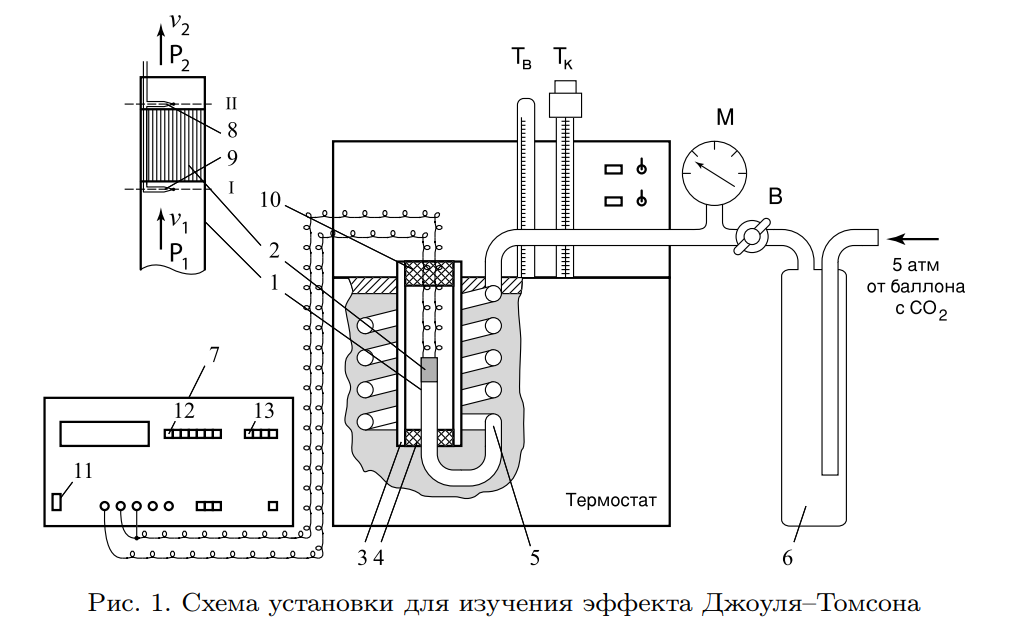
\includegraphics[width = \textwidth]{Рисунок 1.png}
    \end{figure}
    
    Углекислый газ под повышенным давлением поступает в трубку через змеевик 5 из балластного баллона 6. Медный змеевик омывается водой и нагревает медленно протекающий через него раз до температуры воды в термостате. Температура воды устанавливается и поддерживается при помощи контактного термометра $T_{\text{к}}$.
    
    Давление газа в трубке измеряется манометром М и регулируется вентилем В. Так как углекислый газ после пористой перегородки выходит в область с атмосферным давлением, то манометр измеряет перепад давлений на входе и выходе трубки.
    
    Разность температур газа до перегородки и после неё измеряется дифференциальной термопарой медь-константан. Константановая проволока диаметром 0,1 мм соединяет спаи 8 и 9, а медные проволоки того же диаметра подсоединены к цифровому вольтметру 7. Отвод тепла через проволоку столь малого сечения пренебрежимо мал. 
    
    Для уменьшения теплоотвода трубка с пористой перегородкой помещена в трубу Дьюара 3, стенки которой посеребрены для уменьшения теплоотдачи за счёт излучения. Для уменьшения теплопередачи за счёт конвекции один конец трубу Дьюара уплотнён кольцом 4, а другой закрыт пробкой 10 из пенопласта. 

\section{Методика измерений}	

    В процессе Джоуля-Томсона газ испытывает трение внутри пористой перегородки, что приводит к его нагреву. Такие потери энергии могут исказить результаты эксперимента. Таким образом, при проведении опыта необходимо дождаться установления стационарного распределения температуры в трубке. При этом, если теплоизоляция достаточно хороша, газ будет "уносить с собой"\ всё выделенное им тепло.
    
\section{Оборудование}

    Как уже было отмечено выше, разность температур измеряется термопарой, подсоединённой к вольтметру. Погрешность измерений вольтметра составляет $\Delta_U = 0,005\text{ мВ}$.
    
    Манометр, используемые в эксперименте имеет шкалу на 100 делений и предел измерений в $6\frac{\text{кгс}}{\text{см}^2}$. Откуда получаем, что отклонение стрелки прибора на одно деление соответствует изменению давления на 5880 Па (считаем, что $1\text{ кгс} = 9,8\text{ Н}$). Показания с прибора снимались следующим образом: считалось число делений, на которые отклонилась стрелка; это число приводилось к паскалям умножением на 5880 Па; полученное значение делилось на 101300$\frac{\text{Па}}{\text{атм}}$; так получался перепад давлений в атмосферах. Погрешность измерений манометра составляет 0,25 делений, то есть $\Delta_P = 1470\text{ Па} \approx 0,01\text{ атм}$ .

\section{Обработка полученных результатов}
 
    \subsection{Определение коэффициента дифференциального эффекта Джоуля-Томсона}
    
    Измерения проводились следующим образом: для каждого из 5 значений температуры термостата снимались показания с вольтметра при 5 различных значениях давления. Результаты измерений приведены в таблице 1. В данной таблице также приведены значения перепада температуры, рассчитанные по формуле:
    \[\Delta T = \frac{U}{\alpha},\]
    где $\alpha$ - коэффициент, связанный с характеристиками термопары и зависящий от температуры. Значения $\alpha$ при разных температурах приводятся в таблице 2.
    
    По данным таблицы 1 построены графики 1-5, а также для наглядного сравнения прямые с этих графиков изображены вместе на графике 6. Из этих данных согласно методу наименьших квадратов получены значение коэффициентов $k = \frac{\Delta T}{\Delta P}$ дифференциального эффекта Джоуля-Томсона. Они приведены в таблице 3 вместе со случайным погрешностями.
    
    Систематическую погрешность коэффициента $k$ нужно считать по формуле:
    \[\Delta_k = k\sqrt{\left(\frac{\Delta_U}{U}\right)^2 + \left(\frac{\Delta_P}{\Delta P}\right)^2}\]
    В каждой серии измерений (при одной и той же температуре термостата) найдём $\Delta_k$ для каждого давления, а затем усредним по этим давлениям (найдём среднее квадратичное). Полученное значение сложим (квадратично) со случайной погрешностью. Результаты также приведены в таблице 3.
    
    \subsection{Определение констант Ван-дер-Ваальса}
    
    Запишем уравнение \eqref{coeff} с использованием обозначения $\frac{\Delta T}{\Delta P} \equiv k$:
    \[k\left(\frac{1}{T}\right) = \frac{2a}{RTC_p} - \frac{b}{C_p}\]
    
    Так как для углекислого газа $C_P = \frac{7}{2}R$, то последнее выражение принимает вид:
    \[k\left(\frac{1}{T}\right) = \frac{4a}{7R^2}\cdot\frac{1}{T} - \frac{2b}{7R}\]
    Прямая, полученная по методу наименьших квадратов и приближающая последнюю формулу, приведена на графике 7. Для данной прямой получено:
    \[\xi \equiv \frac{4a}{7R^2} = (660 \pm 180)\ \frac{\text{К}^2}{\text{атм}}\]
    \[\eta \equiv \frac{2b}{7R} = (1.1 \pm 0.6)\ \frac{\text{К}^2}{\text{атм}}\]
    Откуда получаем:
    \[a = \frac{7}{4}\xi R^2 = (0,79 \pm 0,21)\ \frac{\text{Па}\cdot\text{м}^6}{\text{моль}^2}\]
    \[b = \frac{7}{2}\eta R = (3,2 \pm 1,7)\cdot10^{-4}\ \frac{\text{м}^3}{\text{моль}}\]
    
    Оценивать систематические погрешности констант Ван-дер-Ваальса не имеет смысла, так как уже случайные погрешности имеют один порядок с этими константами.
    
    Теперь по формуле \eqref{T_inv} найдём температуру инверсии дифференциального эффекта Джоуля-Томсона.
    \[T_{\text{инв}} = \frac{2a}{Rb} = (590 \pm 350)K\]
    Погрешность $T_{\text{инв}}$ рассчитывалась по формуле:
    \[\Delta_T = T_{\text{инв}}\sqrt{\left(\frac{\Delta_a}{a}\right)^2 + \left(\frac{\Delta_b}{b}\right)^2}\]
    

\section{Вывод}

    В ходе данной работы были вычислены коэффициенты дифференциального эффекта Джоуля-Томсона для разных температур, лежащих на промежутке [20,2; 60]\ \degree C. По этим коэффициентам были найдены константы Ван-дер-Ваальса, а также температуру инверсии дифференциального эффекта Джоуля-Томсона.
    В справочных данных автору удалось найти, что для углекислого газа костанты Ван-дер-Ваальса равны
    \[a = 0,36\ \frac{\text{Па}\cdot\text{м}^6}{\text{моль}^2};\ b = 0,43\cdot10^{-4}\ \frac{\text{м}^3}{\text{моль}}\]
    Полученное в ходе работы значение константы $b$ совпадает с табличным в пределах найденной погрешности. Однако того же нельзя сказать о константе $a$. Именно это, по моему мнению, привело к тому, что найденное значение температуры инверсии, не совпадает с теоретическим значением, которое приближённо равняется $2000 K$.
    
    На мой взгляд, основным источником погрешностей в данной работе послужил вольтметр, так как при каждом измерении на его дисплее всего одна/две значащие цифры не менялись, остальные флуктуировали. Также для перепадов давления 2-3 атм в трудом удавалось поддерживать давление постоянным с помощью вентиля: оно изменялось в среднем на половину деления за время одного измерения.
    
    Для увеличения точности эксперимента предлагаю использовать более точные вольтметр (или термопару), а также автоматизировать поддержание постоянства перепада давлений.
    
\newpage
\section{Приложения}

    \subsection{Таблица 1. Результаты измерений.}
    \begin{tabular}{|P{1,25cm}|P{1,5cm}|P{1,25cm}|P{1cm}|P{1,5cm}|}
        \hline
        \multicolumn{5}{| c |}{$\Delta P(U)$ при разных T} \\
        \hline
        № изм. & $\Delta$ P, \text{атм} & U, \text{мкВ} & T, \degree C & $\Delta$T, \degree C \\
        \hline\hline
        \multirow{5}{4em}{1} & 3,95 & 160 & 20,2 & 3,93  \\ \cline{2-5}
        & 3,42 & 130 & 20,2 & 3,19    \\ \cline{2-5}
        & 2,90 & 110 & 20,2 & 2,70    \\ \cline{2-5}
        & 2,38 & 80  & 20,3 & 1,97    \\ \cline{2-5}
        & 1,86 & 60  & 20,3 & 1,47    \\ \hline
        \hline
        
        \multirow{5}{4em}{2} & 3,95 & 150 & 30,0 & 3,61   \\
        \cline{2-5}
        & 3,42 & 120 & 30,1 & 2,88    \\ \cline{2-5}
        & 2,90 & 100 & 30,1 & 2,40    \\ \cline{2-5}
        & 2,38 & 80  & 30,0 & 1,92    \\ \cline{2-5}
        & 1,86 & 50  & 30,0 & 1,20    \\ \hline
        \hline
        
        \multirow{5}{4em}{3} & 3,95 & 140 & 40,0 & 3,29 \\ \cline{2-5}
        & 3,42 & 120 & 40,0 & 2,82    \\ \cline{2-5}
        & 2,90 & 90  & 40,0 & 2,12    \\ \cline{2-5}
        & 2,38 & 70  & 40,0 & 1,65    \\ \cline{2-5}
        & 1,86 & 50  & 40,0 & 1,18    \\ \hline
        \hline
        
        \multirow{5}{4em}{4} & 3,95 & 130 & 50,0 & 3,00\\
        \cline{2-5}
        & 3,42 & 110 & 50,0 & 2,54    \\ \cline{2-5}
        & 2,90 & 90  & 50,0 & 2,08    \\ \cline{2-5}
        & 2,38 & 70  & 50,0 & 1,62    \\ \cline{2-5}
        & 1,86 & 50  & 50,0 & 1,15    \\ \hline
        \hline
        
        \multirow{5}{4em}{5} & 3,95 & 130 & 60,0 & 2,95\\
        \cline{2-5}
        & 3,42 & 100 & 60,0 & 2,27    \\ \cline{2-5}
        & 2,90 & 80  & 60,0 & 1,81    \\ \cline{2-5}
        & 2,38 & 60  & 60,0 & 1,36    \\ \cline{2-5}
        & 1,86 & 40  & 60,0 & 0,91    \\ \hline
    \end{tabular}
    
    \subsection{Таблица 2. Температурная зависимость коэффициента $\alpha$.}
    \begin{tabular}{|c|c|c|c|c|c|}
        \hline
        Температуры, \degree C & 0-10 & 10-20 & 20-30 & 30-40 & 40-50 \\
        \hline
        мкВ/\degree C & 38,9 & 39,8 & 40,7 & 41,6 & 42,5 \\
        \hline\hline
        Температуры, \degree C & 50-60 & 60-70 & 70-80 & 80-90 & 90-100 \\
        \hline
        мкВ/\degree C & 43,3 & 44,1 & 44,9 & 45,6 & 46,4 \\
        \hline
    \end{tabular}
    
    \subsection{Таблица 3. Коэффициент дифференциального эффекта Джоуля-Томсона при разных температурах.}
    \begin{tabular}{|c|c|c|c|c|}
         \hline
         T,\ \degree C & k, К/атм & $\Delta_k^{\text{случ}}$, К/атм & $\Delta_k^{\text{сист}}$, К/атм & $\Delta_k$, К/атм\\ \hline 
         \hline
         20,2 & 1,18  & 0,04  & 0,066 & 0,08 \\ \hline
         30   & 1,11  & 0,05  & 0,069 & 0,09 \\ \hline
         40   & 1,03  & 0,04  & 0,067 & 0,08 \\ \hline
         50   & 0,885 & 0,003 & 0,058 & 0,07 \\ \hline
         60   & 0,96  & 0,05  & 0,075 & 0,09 \\ \hline
    \end{tabular}
    
    \subsection{График 1. При температуре T = 20,2\ \degree C.}
    \begin{center}
        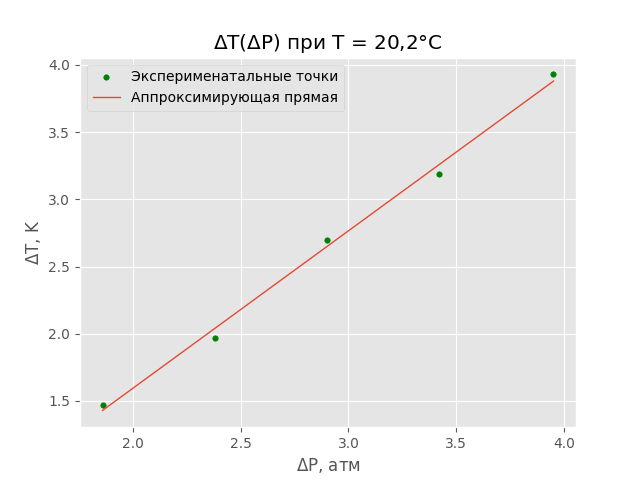
\includegraphics[width=9cm]{20.png}
    \end{center}
    
    \subsection{График 2. При температуре T = 30\ \degree C.}
    \begin{center}
        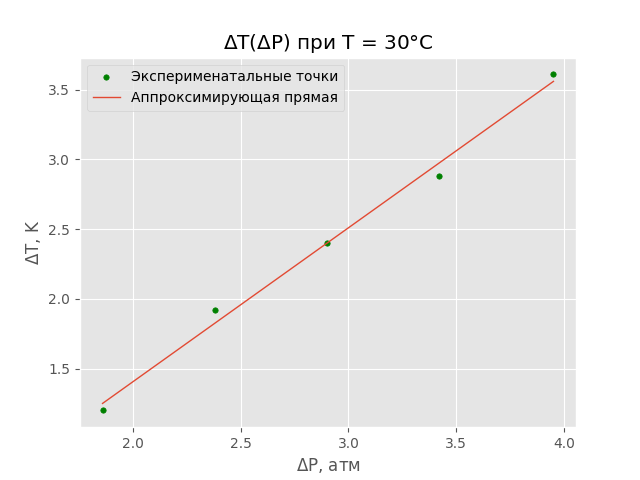
\includegraphics[width=9cm]{30.png}
    \end{center}
    
    \subsection{График 3. При температуре T = 40\ \degree C.}
    \begin{center}
        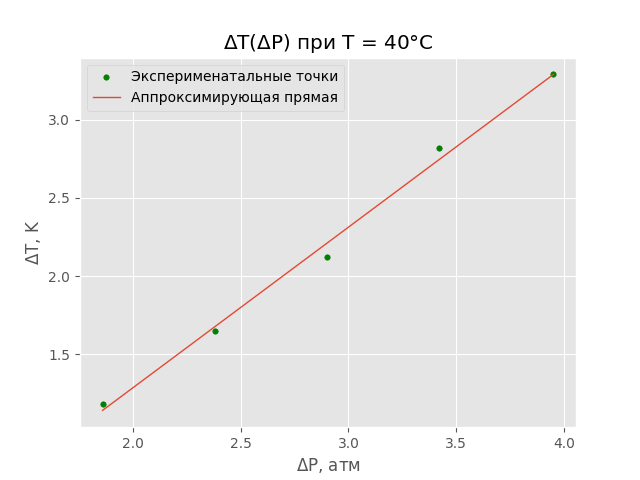
\includegraphics[width=9cm]{40.png}
    \end{center}
    
    \subsection{График 4. При температуре T = 50\ \degree C.}
    \begin{center}
        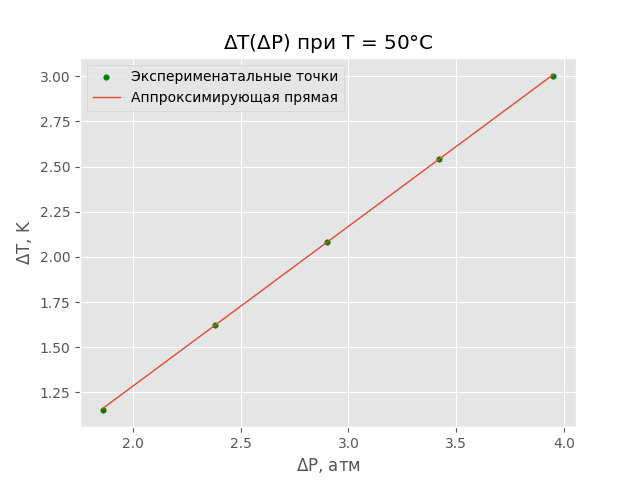
\includegraphics[width=9cm]{50.png}
    \end{center}
    
    \subsection{График 5. При температуре T = 60\ \degree C.}
    \begin{center}
        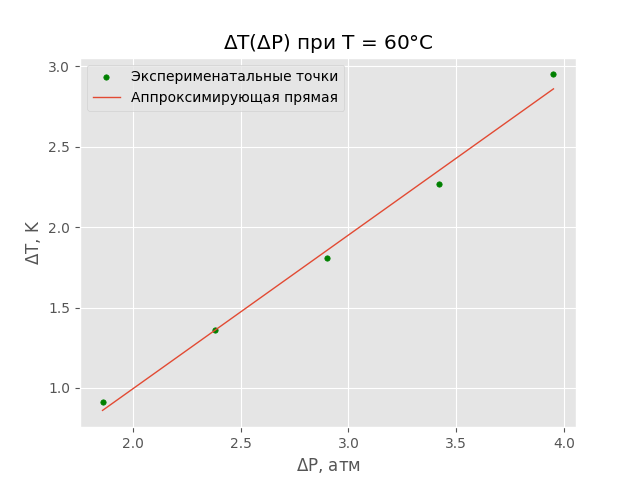
\includegraphics[width=9cm]{60.png}
    \end{center}
    
    \subsection{График 6. Сравнение зависимостей при разных температурах.}
    \begin{center}
        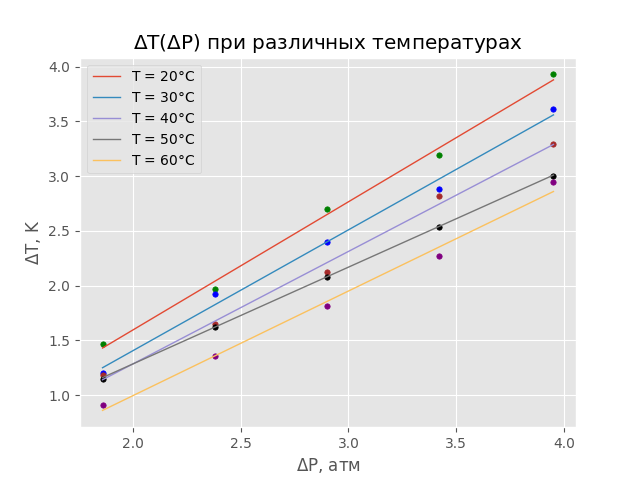
\includegraphics[width=\textwidth]{All.png}
    \end{center}
    
    \subsection{График 7. Поиск констант Ван-дер-Ваальса.}
    \begin{center}
        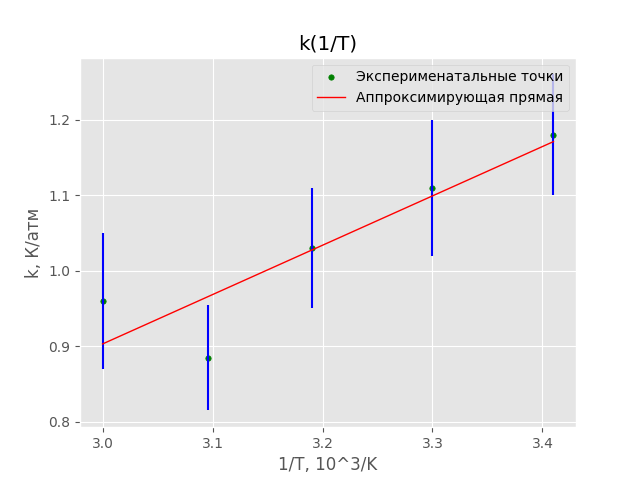
\includegraphics[width=\textwidth]{Van_der_Waals_2.png}
    \end{center}


\end{document}